\section{Results}
\label{05}
In this section, we discuss how well different versions of our robot played against some sample robots provided with the Robocode installation. We also present data gathered while testing as well as evaluate the significant differences between each robot (if any).

\subsection{Test Set-Up}
We tested four different set-ups of the robot versus four different sample robots. Each test consisted of 10 tests of a 10-round battle with otherwise default Robocode rules. In order to test the effect of each setting, we only changed a single setting in each variation of our robot from our default robot. Because of the large number of different possible combination of settings, it is likely that we have not found the best possible one. The settings for our robots can be seen in table \ref{table-robotsettings}.

\subsubsection{Enemy Robots} 
We tested our robot against the \textit{MyFirstRobot}, \textit{SittingDuck}, \textit{Spinbot}, and \textit{Tracker} sample robots. \textit{MyFirstRobot} moves in a see-saw motion, rotates its gun and fires whenever it scans another robot. \textit{Spinbot} moves in a circular motion and fires a powerful shot whenever it scans an enemy. The \textit{Tracker} robot scans for a target, locks on to it, moves close and then fires at the target. As the name suggests, the \textit{SittingDuck} takes no action, does not move and does not react. It is often used to test how well the guns of a robot works.

We have not provided tables and data sets for the results of our tests versus the \textit{SittingDuck} robot, as we obtained a 100\% score against it with all four versions of the MCTS robot on every trial. 

\begin{table}
\begin{center}
\renewcommand{\arraystretch}{1}
\caption{Robot settings for score rewards}
\label{table-robotsettings}
\begin{tabular}{|c | c | c |c |}
\hline
Robot & Movement & Turning & Shooting\\
\hline
Default & 1.5 & 0.4 & 0.1\\
\hline
MCTS-1 & \textbf{3.0} & 0.4 & 0.1\\
\hline
MCTS-2 & 1.5 & \textbf{0.8} & 0.1\\
\hline
MCTS-3 & 1.5 & 0.4 & \textbf{0.2}\\
\hline
\end{tabular}
\end{center}
\end{table}

\subsubsection{Default-MCTS Robot}
We established the baseline "Default" robot settings by trying out different settings and deciding on a combination that seemed to be somewhat successful. The settings used for this robot offer a good compromise between shooting, moving, and turning. This default robot is somewhat trigger happy, however, and at times attempts to shoot every time it is possible.

\subsubsection{MCTS-1}
This robot should prioritize movement more than it ended up doing. It is, however, difficult to truly evaluate how much more it moves without tracking it specifically, which we did not. 

\subsubsection{MCTS-2} 
This robot is highly rewarded for turning around, which causes it to spin wildly while it shoots seemingly at random. It is possible that the doubling of the turning reward was too much and it would have been more useful to test with less of an increase (or perhaps even a decrease).

\subsubsection{MCTS-3}
We had anticipated that this robot would shoot more than the default robot, but we did not notice any apparent difference in the amount of shots fired. This is likely due to the trigger happiness of the default robot; if it already shoots as often as it can, then increasing the shooting reward is unlikely to make much of a difference.

\subsection{Data}
The scoring data in this section is represented as percentages of the total score in a single battle, e.g. our robot got 25\% of the total points and the enemy robot got the remaining 75\%. We represent it as such because of the stochastic nature of spawning positions and robot heading at the start of a round. By comparing percentage of the scores instead of absolute values, we are letting these random factors influence the results in the least possible way.

\subsubsection{Default-MCTS Robot}
As the default-MCTS robot was the baseline for our tests, we have done all significance comparisons using the test data for this robot.

Table \ref{table-default-score} indicates large differences in performance against the three different enemy robots. While the default robot never gets below 23\% score against \textit{MyFirstRobot}, it does poorly against the \textit{Spinbot} and even worse against the \textit{Tracker} robot. Interestingly, the robot is consistently poor against the \textit{Tracker} robot, as evidenced by the lower standard deviation (and seen on figure \ref{figure-BarGraph}\footnote{The variance bars on the graph represent standard deviation.}).

The distribution of scores against the enemy robots are shown in figures \ref{figure--Distribution-MFR}, \ref{figure--Distribution-Spinbot}, and \ref{figure--Distribution-Tracker}. The values are the decimal representations of the percentage scores achieved by the default robot. While the scores mostly fit somewhat nicely around the bell curve, the results against both \textit{MyFirstRobot} and \textit{Spinbot} have one rather extreme outlier.

\begin{table}
\begin{center}
\renewcommand{\arraystretch}{1.3}
\caption{Score for the Default-MCTS Robot}
\label{table-default-score}
\begin{tabular}{|c | c | c |c | c| c |}
\hline
Enemy & Mean & Median & Mode & Std. Dev & Std. Err.\\
\hline
MyFirstRobot & 25.6\% & 25.4\% & None & 1.609 & 0.509\\
\hline
Spinbot & 15.7\% & 16.3\% & None & 2.145 & 0.678 \\
\hline
Tracker & 10.8\% & 10.5\% & None & 0.779 & 0.246 \\
\hline
\end{tabular}
\end{center}
\end{table}

\begin{figure}[htp]
\centerline{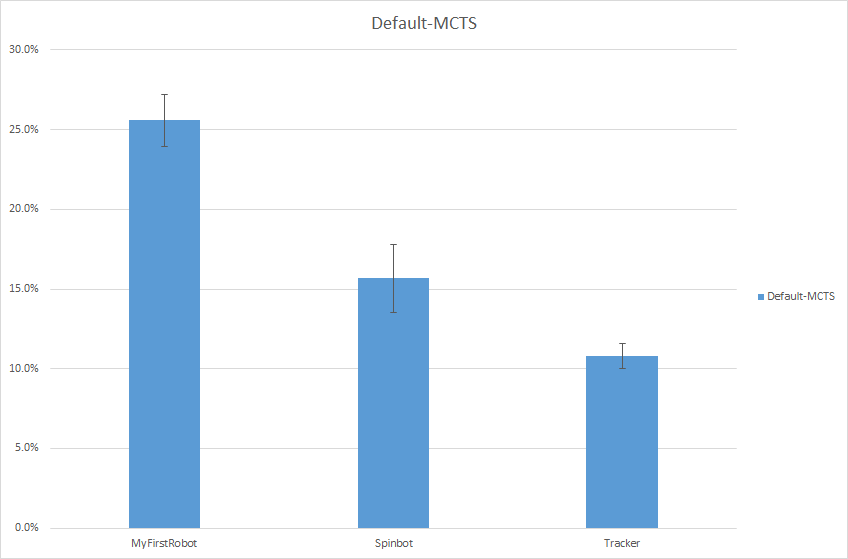
\includegraphics[width=\columnwidth]{Images/BarGraph}}
\caption{Mean score percentages for the Default MCTS controller.}
\label{figure-BarGraph}
\end{figure}

\begin{figure}[htp]
\centerline{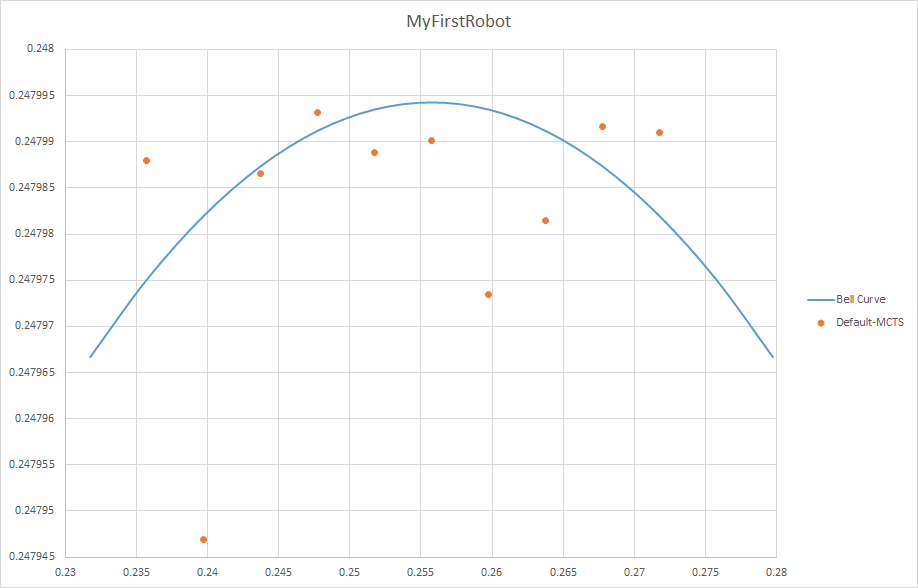
\includegraphics[width=\columnwidth]{Images/MyFirstRobotDistribution}}
\caption{Distribution of results by default-MCTS against the "MyFirstRobot".}
\label{figure--Distribution-MFR}
\end{figure}

\begin{figure}[htp]
\centerline{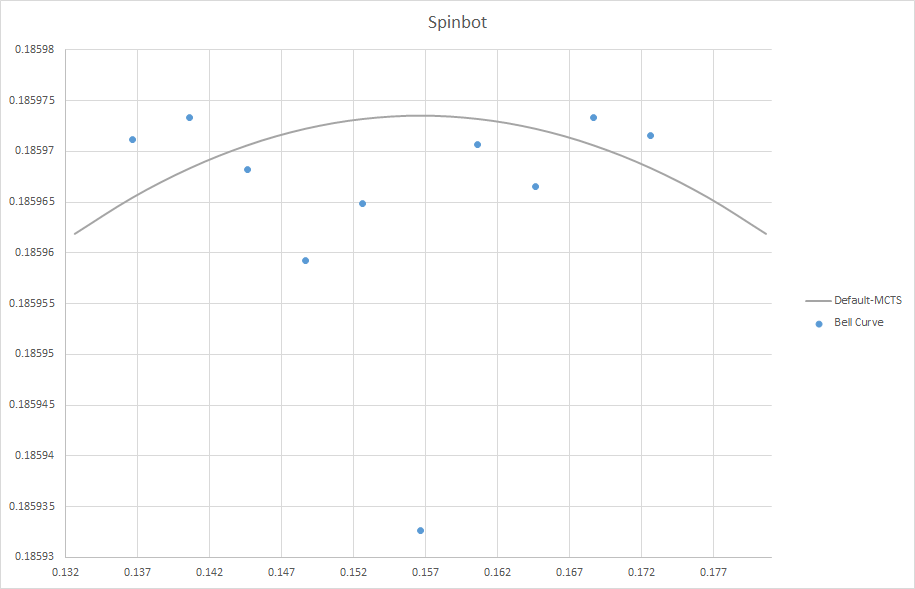
\includegraphics[width=\columnwidth]{Images/SpinbotDistribution}}
\caption{Distribution of results by default-MCTS against the "Spinbot" robot.}
\label{figure--Distribution-Spinbot}
\end{figure}

\begin{figure}[htp]
\centerline{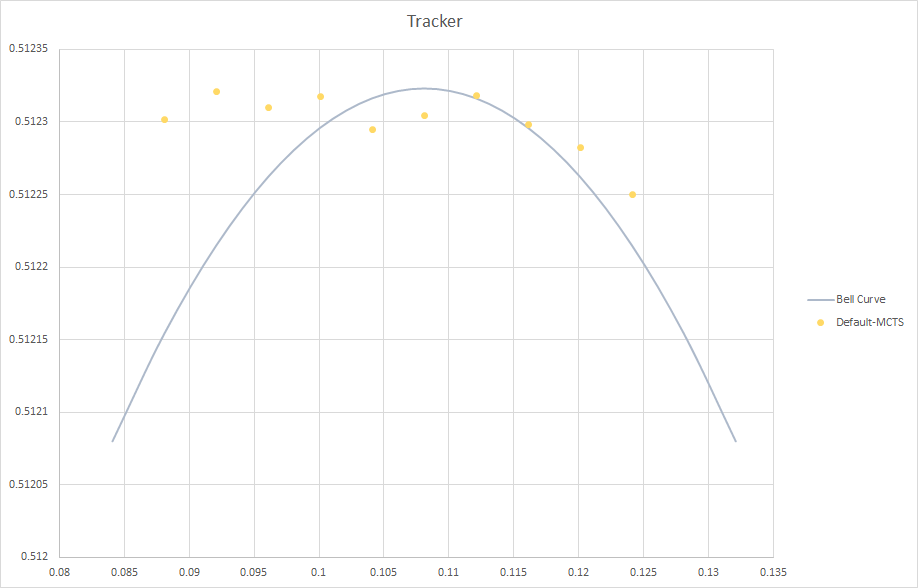
\includegraphics[width=\columnwidth]{Images/TrackerDistribution}}
\caption{Distribution of results by default-MCTS against the "Tracker" robot.}
\label{figure--Distribution-Tracker}
\end{figure}

\subsubsection{Other versions}
Tables \ref{table-MCTS1-score}, \ref{table-MCTS2-score}, and \ref{table-MCTS3-score} show the scores of the three variations of our robot. As shown by tables \ref{table-MFS-significance}\footnote{The variances were not equal between Default and MCTS-3, so a different critical t-value was used.}, \ref{table-spinbot-significance}, and \ref{table-tracker-significance}, two of the robot variations have significant differences in score percentage. MCTS-1 performs significantly better against the \textit{Spinbot} and the \textit{Tracker} robot, but not so against \textit{MyFirstRobot}. MCTS-2 performs significantly worse against all three enemy robots.

\begin{table}
\begin{center}
\renewcommand{\arraystretch}{1.3}
\caption{Score for the MCTS-1 Robot}
\label{table-MCTS1-score}
\begin{tabular}{|c | c | c |c | c| c |}
\hline
Enemy & Mean & Median & Mode & Std. Dev & Std. Err.\\
\hline
MyFirstRobot & 27.2\% & 26.6\% & None & 3.292 & 1.041\\
\hline
Spinbot & 19.5\% & 19.3\% & None & 2.437 & 0.771 \\
\hline
Tracker & 13.7\% & 13.9\% & 14.3 & 1.789 & 0.567 \\
\hline
\end{tabular}
\end{center}
\end{table}

\begin{table}
\begin{center}
\renewcommand{\arraystretch}{1.3}
\caption{Score for the MCTS-2 Robot}
\label{table-MCTS2-score}
\begin{tabular}{|c | c | c |c | c| c |}
\hline
Enemy & Mean & Median & Mode & Std. Dev & Std. Err.\\
\hline
MyFirstRobot & 8.4\% & 8.3\% & None & 1.854 & 0.586\\
\hline
Spinbot & 3.4\% & 3.6\% & 3.7 & 0.970 & 0.307  \\
\hline
Tracker & 4.4\% & 4.5\% & 4.6 & 0.491 & 0.155 \\
\hline
\end{tabular}
\end{center}
\end{table}

\begin{table}
\begin{center}
\renewcommand{\arraystretch}{1.3}
\caption{Score for the MCTS-3 Robot}
\label{table-MCTS3-score}
\begin{tabular}{|c | c | c |c | c| c |}
\hline
Enemy & Mean & Median & Mode & Std. Dev & Std. Err.\\
\hline
MyFirstRobot & 26.0\% & 25.8\% & None & 3.054 & 0.965\\
\hline
Spinbot & 15.9\% & 15.1\% & None & 3.319 & 1.049  \\
\hline
Tracker & 11.4\% & 11.1\% & None & 1.303 & 0.413 \\
\hline
\end{tabular}
\end{center}
\end{table}


\begin{table}
\begin{center}
\renewcommand{\arraystretch}{1}
\caption{Significance test using the MyFirstRobot Robot}
\label{table-MFS-significance}
\begin{tabular}{|c | c | c |c | c | c |}
\hline
Controller & Mean & Variance & t-value & critical t & Significant\\
\hline
Default & 0.256 & 0.00025 & N/A & N/A & N/A\\
\hline
MCTS-1 & 0.272 & 0.00108 & 1.397 & 2.101 & No\\
\hline
MCTS-2 & 0.084 & 0.00034 & -22.067 & 2.101 & Yes\\
\hline
MCTS-3 & 0.260 & 0.0009 & 0.354 & 2.145 & No\\
\hline
\end{tabular}
\end{center}
\end{table}

\begin{table}
\begin{center}
\renewcommand{\arraystretch}{1}
\caption{Significance test using the Spinbot Robot}
\label{table-spinbot-significance}
\begin{tabular}{|c | c | c |c | c | c |}
\hline
Controller & Mean & Variance & t-value & critical t & Significant\\
\hline
Default & 0.157 & 0.00046 & N/A & N/A & N/A\\
\hline
MCTS-1 & 0.195 & 0.00059 & 3.730 & 2.101 & Yes\\
\hline
MCTS-2 & 0.034 & 0.00009 & -16.502 & 2.101 & Yes\\
\hline
MCTS-3 & 0.159 & 0.00110 & 0.215 & 2.1001& No\\
\hline
\end{tabular}
\end{center}
\end{table}

\begin{table}
\begin{center}
\renewcommand{\arraystretch}{1}
\caption{Significance test using the Tracker Robot}
\label{table-tracker-significance}
\begin{tabular}{|c | c | c |c | c | c |}
\hline
Controller & Mean & Variance & t-value & critical t & Significant\\
\hline
Default & 0.108 & 0.00006 & N/A & N/A & N/A\\
\hline
MCTS-1 & 0.137 & 0.0003 & 4.744 & 2.101 & Yes\\
\hline
MCTS-2 & 0.004 & 0.00002 & -22.067 & 2.101 & Yes\\
\hline
MCTS-3 & 0.114 & 0.00017 & 1.229 & 2.101 & No\\
\hline
\end{tabular}
\end{center}
\end{table}

\subsection{Evaluation}
As noted above, MCTS-1 performs significantly better than our default-MTCS against two of the three enemy robots. It also averages a better score against the last of the three robots, although this difference is not significant. Thus we can conclude that MCTS-1 is the best of the four robots tested for this paper, default-MCTS and MCTS-3 are about equal, and by far the worst is MCTS-2, which performs horribly against all three enemies.

%which robot was best
\subsubsection{Speed}
The speed of the algorithm is capped at 10 milliseconds per iteration in order to avoid skipping any turns in Robocode. This does not allow the algorithm to search very deeply into the tree, but we believe this to be a somewhat positive behaviour. Because the simulation of the game state and the assumptions we make about the actions taken by the opponent can potentially be wildly inaccurate, we will rarely benefit from simulating too far into the future.
